\documentclass[10pt]{article}

\usepackage{graphicx}

\begin{document}

\title{Coordinating parallelism between build systems and compilers to enable project builds to better scale on modern machines}
\author{Sarah Spall}
\date{}
\maketitle

\section{Introduction}

In today's world multi-core machines are ubiquitous, with machines having up to 64 real cores.
Having a machine with 64 cores instead of 32 cores isn't useful however, if the software running
on it isn't capable of utilizing the 32 additional cores.  In the realm of parallel programming
research, one maybe neglected area is build systems and compilers.  Even though every developer
uses a build system and a compiler, not much research has been done to ensure both are as
parallel as possible.

% What is the high level thing I want to say?
The build systems and compilers of today tend to work separately even though they are
solving separate parts of the same problem.  The build system is usually responsible for coordinating
thes sequential tasks that make up a project build; these sequential tasks are often
compilation jobs.  On the other hand, the compiler is responsible for completing some of the sequential
tasks that the build system is waiting on.  Traditionally, independent compilation jobs can be
launched in parallel by the build system if they do not depend on one another, but internally,
they are not themselves run in parallel.

I propose the following thesis: \emph{By combining and coordinating parallelism at the build system level
and at the compiler level, project builds can better scale on modern day multi-core
machines.}

In support of this thesis I plan to do the following things.  First, I will analyse the parallelism
currently exposed and observed in existing projects.  Second, I will investigate ways to expose
additional parallelism at the build system level.  Third, I will work towards discovering methods
that will make writing a paralle compiler realistic, and show that a parallel compiler could work
in concert with a build system to build projects as quickly as possible.  In the following
sections of this proposal I will explain how I plan to accomplish these things in more detail.

\section{Current state of build systems and compilers}
\label{sec:state}
% Start out talking about multiple build systems and how they general all work
% Then move onto the specifics of Make itself.

% List of build systems: Make, Shake, Bazel, Buck, Ninja, 

There are many existing build systems whose general goal is to build a project as quickly as
possible.  Some of these build systems include: Make \cite{feldman1979make}, Shake
\cite{mitchell2012shake}, Bazel \cite{bazel}, Buck \cite{buck}, and Ninja \cite{ninja}.
All of these build systems will launch independent tasks in parallel as one method of building a
project as quickly as possible.

Buck appears to go beyond this model of exploiting only the obviously available parallelism.  
Usually it is entirely the user of the build system's job to fully define which tasks are independent.
Buck claims to not require users to fully define which tasks are independent and will break coarse-build rules
up into smaller independent pieces that can be built in parallel.  

Make is a ubiquitous build system that first uses the information specified  in a
Makefile to construct a directed graph of a build project's tasks.  Make then performs a
topological sort on the graph to determine the order to build the targets.  Programmers can
specify which tasks
for a specific target may safely be run in parallel by specifying them as dependencies of the
target, or by writing a line such as \emph{make one two three}.  Make lets users specify how many
jobs may run at once, but of course how many jobs will run in parallel is directly dependent on the amount
of parallelism available in the project's directed graph.   We would like to go
beyond this model of build-level parallelism and discover more parallelism within the compilation jobs
launched by the build system.

% not sure if this note about shake really fits here
%shake has an interesting strategy for reducing contention for system resources such as IO and
%memory; which is to run tasks in a random order.  They believe that it is more likely that tasks
%which are close together are more likely to use the same system resources.

% Make lets users to -j n; so can build independent targets in parallel; where the independence
% of any number of targets is defined by the user.

% Shake is the haskell build system which..... also allows independent rules at the same time
% shake has a thread pool and rules are added to a queue to be run by the thread pool.
% which I believe is just about the same as Make and probably every system
% user can specify max number of rules run in parallel
% shake says it ensures max parallelism by launching a temporary worker when a rule is blocked
% waiting on dependencies; why does this ``ensure'' max parallelism?
% run tasks in a random order to reduce contention for system resources

% bazel is google's build system
% says you can set it up to run ``in a highly parallel and incremental fashion''
% bazel has a -j option which says it allows the user to specify the number of jobs that should
% be executed CONCURRENTLY; the scheduler tries to avoid running more concurrent jobs if
% it will negatively affect resource usage 
% bazel claims it allows builds to scale by caching and remote execution.
% What do they mean by scale?  To larger and larger projects?  Prob don't mean scale to use
% many many cores

% buck is facebook's build system
% buck says it constructs a DAG and then can easily know what can be built in parallel;
% like make
% Buck acknowledges this fact ``This execution model means that breaking modules into finer
% dependencies creates opportunities for increased parallelism, which improves throughput.''
% buck uses something they call ``graph enhancement'' to expose more parallelism
% graph enhancement can break up a larger task into smaller ones that can be done in parallel
% graph enhancement can also move dependnecy edges.
% not sure what kind of analysis they do to determine this; maybe its very shallow or very
% intelligent
% should look at source code
% action graph is only built once; unless dependencies in buid file change

% ninja; built by some guy at google?
% builds are always run in parallel; so just like every other project.  by default

% talk about parallel compilation now

Although there is not parallel production compiler, to the best of my knowledge, research
has been done on how to parallelize certain compiler passes.  These passed include
parsing \cite{}, register allocation \cite{}, program analysis \cite{}, and typechecking \cite{}.
% need to say more


% Why didn't these things make it into production compilers?

% maybe the following sentence belongs in the next section?
%It is generally considered difficult to write good parallel programs, so much work has gone into
%providing developers with tools for analysing the parallelism in their programs [citations].  

% say how builds create a graph then run things in parallel based on dependency info
% but most of those tasks being run are sequential processes


% I should probably validate the above claim

% want to go beyond this model

% Ask ryan about using his 1 versus 16 core debian build parallelism

\section{Parallel analysis tool for build systems}

\begin{figure}[t]
  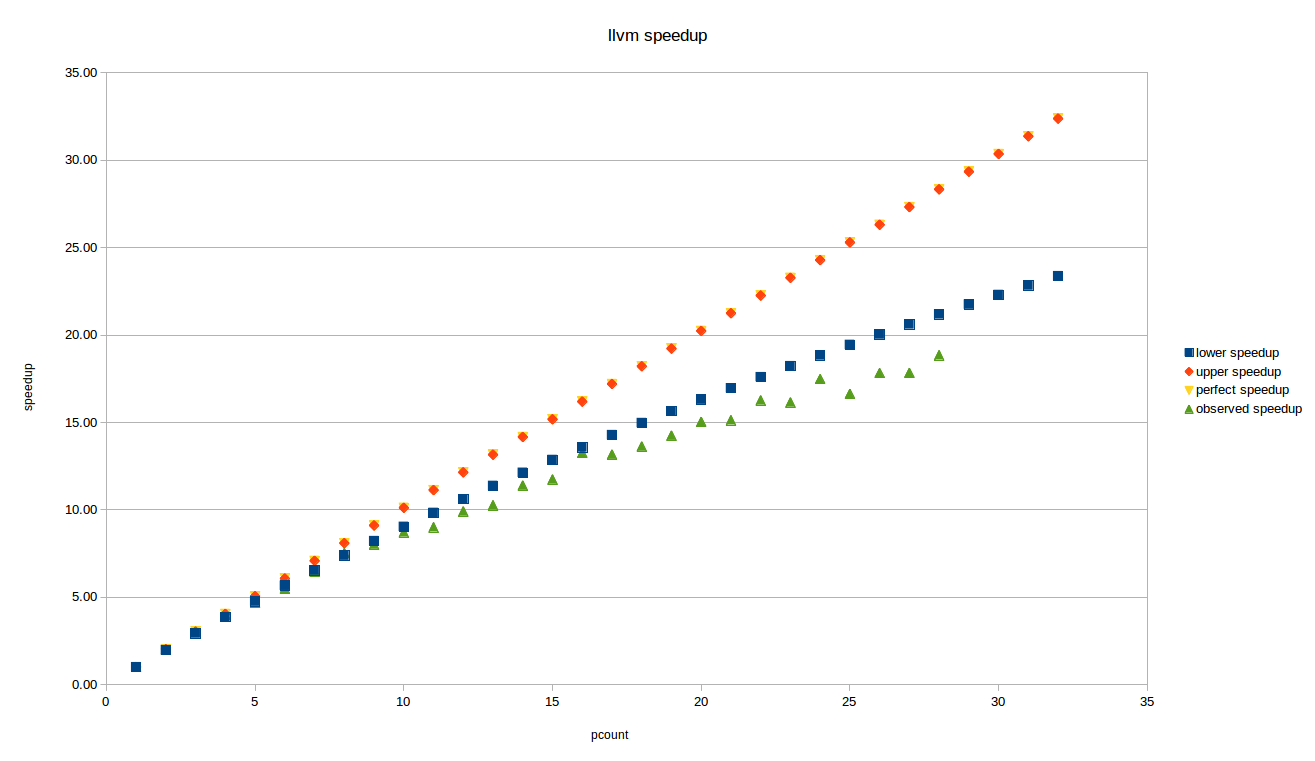
\includegraphics[height=6.5cm]{llvm-speedup-chart.png}
  \caption{Building LLVM on 1 to 28 cores.}\label{fig:llvm}  % update this with to 32 cores
\end{figure}

\begin{figure}[t]
  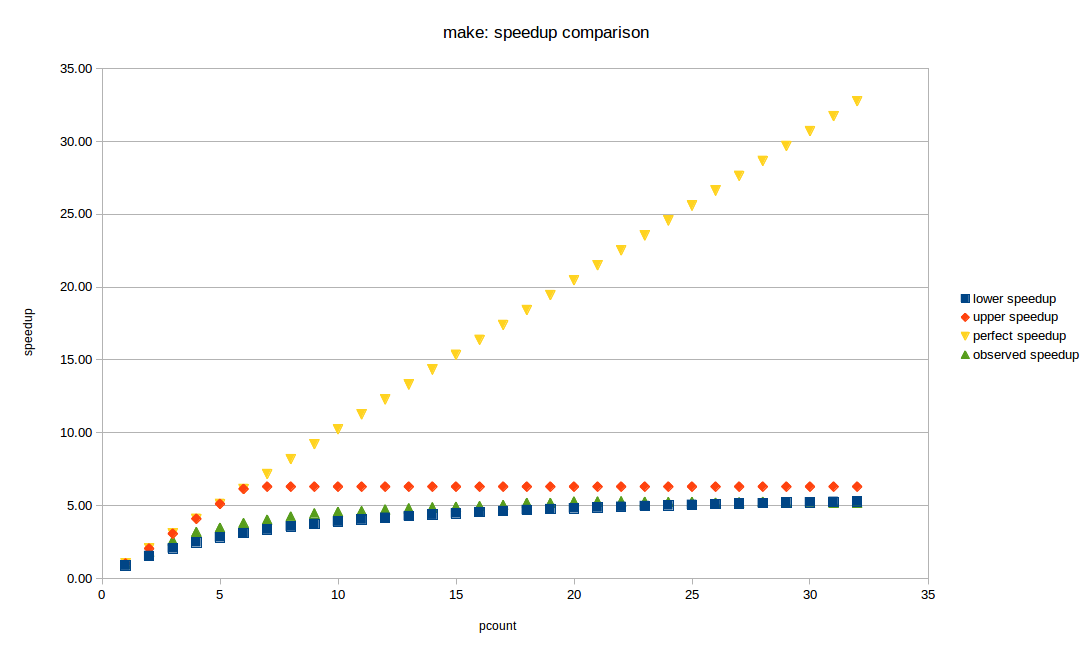
\includegraphics[height=6.5cm]{make-speedup-comparison.png}
  \caption{Building GNU Make on 1 to 32 cores.}\label{fig:make}
\end{figure}

Due to the difficulty of writing good parallel programs, many tools have been created to analyse
parallel programs.  Cilkprof \cite{schardl2015cilkprof}, Kremlin \cite{garcia2011kremlin}, and
TaskProf \cite{yoga2017fast} are a few of these tools.  Cilkprof is a profiler for multithreaded
Cilk programs and by collecting work and span information for every call site in a program,
it can identify bottlenecks and help programmers manually improve their parallel programs.  Similarly,
Taskprof identifies which areas of a task parallel program should be optimized to improve
parallelism.  Kremlin, on the other hand, analyses a sequential version of a program to make
suggestions of which portions should be parallelized first.

Even though a project build is just a specialized version of a parallel program, to the best of
my knowledge, there is no parallel analysis tool that can help analyse a project build.  In the spirit of
previous parallel analysis tools, I propose such a tool for Make.  This tool will
serve two main purposes; first, it will help us analyse and understand the current state of
parallelism in project builds that use Make, and second, it will assist programmers in understanding
the parallelisism available in their project builds and will be able to make suggestions of which
targets and rules could be rewritten to expose more parallelism.

Work has already begun on this analysis tool and it has already been used to analyse the builds of
projects such as LLVM \cite{lattner2002llvm} and GNU Make \cite{gnumake}.  The tool works by first recording information from a
run of GNU Make and then during a post-mortem
analysis rebuilding the DAG built by Make.  From this DAG we can learn the work, span, and
parallelism of the project.  From this we can predict how long it will take to build
the project on any number of cores, as well as identify which portions of the Makefile the
developer may wish to re-evaluate.
% brief overview of how these 3 tools work.

From our analysis of LLVM and GNU Make, we have observed two different parallelism stories.
See figure~\ref{fig:llvm} on page~\pageref{fig:llvm} to see the speedups predicted and
observed when building LLVM on
1 core all the way to 28 cores.  Using Brent's law \cite{brent1974parallel} and the work and span
calculations, we can predict the upper expected speedup and the lower expected speedup bounds.
In this case, upper speedup, red diamonds, and perfect speedup, yellow triangles, are the same.
This is because LLVM exposes ample parallelism, with a predicted parallelism of 82; which means that
we would expect LLVM's build to run 82x faster on an infinite number of processers than on a single
processor.  In this chart we can see the lower expected speedup is indicted by a blue square, and
the actual observed speedup, green triangle, falls slightly below this when run about 10 to 28
cores.  So, here we see that LLVM fails to scale on 28 cores even though there is ample exposed
parallelism.  We predict this is due to contention for system resources.

Building GNU Make tells a different story.  Refer to figure~\ref{fig:make} on page ~\pageref{fig:make}
to see the speedups predicted and observed when building GNU Make on 1 to 32 cores.  Unlike with
LLVM, GNU Make's build does not expose ample parallelism and has a parallelism of only 6.  The
flattening of the upper speedup line, red diamonds, is due to the parallelism of the project being
only 6.  The best way to speedup GNU Make's build would be to try and decrease it's span.

% figure for llvm....
% A lot of available parallelism, but not being used
% hypothesis: problem is in competing for IO and memory so, move parallelism to compiler
% to alleviate this

% figure for ocaml?
% Not enough available parallelism?


\section{Parallel compilers}

% parallelizing compilers; gibbon paper; better representations for parallelizing compilers
% paralle lvars?

% Move on to parallel compilers and the lack of parallel compilation.....  Still need to motivate
% this and I suppose the build stuff
Many of the long sequential tasks launched by a build system are compilation jobs.  Thus, to
expose additional parallelism beyond what can be exposed at the build system level, an at least
partially parallel compiler is necessary.  A parallel compiler could decrease the span
of a previously sequential task and thus potentially decrease the span of the project build as a
whole.  Additionally, for projects that are failing to scale as well as their available parallelism
predicts they should, it may prove useful to move some of that parallelism to a different area.
For example, maybe 16 threads all reading different files is putting too much pressure on the file
system and causing excessive overhead, but having 4 groups of 4 threads operate on 4 different files
in parallel, might increase observed parallelism by decreasing resource contention.

% Certainly what Shake does is also work considering doing but I'm not sure best way to work that in atm

To validate this hypothesis we can measure the utilization of various system resources when
a representative project is built with exclusively build-level parallelism and when a
the same project is built with a mix of build-level and compilation-level parallelism.  Resource utilization
could then be compared to predicted speedups and observed speedups.  If moving soe of the parallel work
to the compilation-level releaved contention, we would expect to see lower resource utilization for the
seconds benchmark for some resources, as well as increased observed parallelism.

% should I explain what different results owuld mean?

In section \ref{sec:state} I mentioned previous work that has been done on parallelizing various compiler
passes and here I will discuss some work we have already done in this direction. 

In our work on the Gibbon compiler \cite{vollmer2017compiling}, we showed that transforming trees into a serialized
format and transforming the code that operates on those tres to operate on the serialized format,
results in a major performance improvement.  We believe this serialized tree format could be used to
write parallel compiler passes.  When the parallel version of a Gibbon benchmark was compared to
GHC running the same parallel benchmark, it was observed that for large trees, a speedup of
11x was observed on 16 cores when compared to a sequential execution.  And, it was observed that GHC
failed to scale beyond 8 cores due to time spent in the garbage collector.  Due to the speedup from
the serialization format itself and the lessened demands on memory allocation we believe Gibbon
could be used to write a performant parallel compiler pass.

% probably butchered that explanation

\section{Scheduler for coordination between build system and compilers}

When exploiting parallelism at both the build-level and at the compiler-level, it may be possible to
decrease observed parallelism by launching too many processes or threads.  In order for the build
system and the compiler to work together as one, a scheduler with a view of the entire system
is necessary.  This scheduler should detect when it is appropriate to run parallel compilation
jobs, and when there is enough parallelism available at the build level to make that unnecessary.
There are of course additional things that could be taken into account, such as: information about which
paths contributed to the span in previous runs could help determine how
to distribute the parallelism in future runs.
For example, Maybe compiling file B takes x
seconds, and would take half that time if parallelized, but if compiling x didn't contribute to
the overall span, then there would be no observed benefit from running that task in parallel.

\section{Conclusion}

In conclusion, I propose the following thesis: \emph{By combining and coordinating parallelism at the build system level
and at the compiler level, project builds can better scale on modern day multi-core
machines.}  And, in support of this thesis I propose analysing and improving the parallelism available in Make builds,
discovering methods for parallelizing compiler passes, and showing that with a scheduler to coordinate parallelism at
the build-level and compiler-level project builds can scale better on modern multi-core machines.

\newpage
\bibliography{citations}
\bibliographystyle{ieeetr}

\end{document}
